%% LyX 2.0.5.1 created this file.  For more info, see http://www.lyx.org/.
%% Do not edit unless you really know what you are doing.
\documentclass[usenatbib]{article}
\usepackage[latin9]{inputenc}
\usepackage[a4paper]{geometry}
\geometry{verbose}
\usepackage{color}
\usepackage{float}
\usepackage{url}
\usepackage{amssymb}
\usepackage{graphicx}

\makeatletter

%%%%%%%%%%%%%%%%%%%%%%%%%%%%%% LyX specific LaTeX commands.
%% A simple dot to overcome graphicx limitations
\newcommand{\lyxdot}{.}


%%%%%%%%%%%%%%%%%%%%%%%%%%%%%% Textclass specific LaTeX commands.
\usepackage{jcappub}

%%%%%%%%%%%%%%%%%%%%%%%%%%%%%% User specified LaTeX commands.






%%%%%%%%%%%%%%%%%%%%%%%%%%%%%% LyX specific LaTeX commands.
%% A simple dot to overcome graphicx limitations
%Make my life significantly easier
\global\long\def\bd{{\bm{\delta}}}

\usepackage{astrobib_mnras2e}

\bibliographystyle{JHEP}

\makeatother

\begin{document}

\title{The Maximum Circular Velocity Dependence of Halo Clustering}

\maketitle

\section{Introduction}

\textcolor{black}{The halo models provide a connection between dark
matter halos and galaxies, and it has been remarkably successful in
describing observations of galaxy clustering. In particular,} the
Halo Occupation Distribution (HOD) and the Conditional Luminosity
Function (CLF) are the two most widely used models of the galaxy-halo
connection. In order to populate halos with galaxies, the HOD gives
the probability $P(N|M)$ that a halo with mass $\mbox{M}$ hosts
$N$ galaxies, while the CLF models the mean abundance $\Phi(L|M)$
of galaxies with luminosity $L$ which live in a dark matter halo
of mass $M$. Those two models are convertible because they operate
under the same assumption; we can obtain an HOD by integrating the
CLF against luminosity and a CLF by differentiating the HOD with respect
to luminosity. Both models have been applied extensively to observations
in order to study the halo-galaxy connection {[}XXX{]} as well as
cosmology {[}XXX{]}.

The halo clustering in large N-body simulations, however, exhibits
dependence on additional halo properties besides halo mass {[}XXX{]}.
Ref.XXX shows that formation time of halos affects to halo bias; older
halos cluster more strongly than younder ones. This additional dependence
of halo clustering is called halo assembly bias, because those additional
dependences come from different assmebly history of halos. \textcolor{black}{If
the galaxy properties in halos are affected by halo environment, the
galaxy occupation statistics will depend on other halo properties
XXX. Several groups study the correlation between galaxy formation
and halo assembly bias both theoretically (Croton et al. 2007) and
observationally (XXX). Even though }\textcolor{red}{Ref. XXX{[}Croton
et al. 2007{]}}\textcolor{black}{{} shows the significant influence
of halo assembly bias on galaxy clustering, there have been mixed
responses to the detection of such a correlation observationally.}

As a response to halo assembly bias, a recent trend in connecting
halos and galaxies has been to use the Abundance Matching technique.
In the Abundance Matching technique, a monotonic relation between
galaxy luminosity and the maximum circular velocities of halos is
assumed so that one can assign the most luminous galaxy to the halo
which have the largest maximum circular velocity and repeat the same
procedure in a hierarchical manner. The motivation behind the technique
is that the maximum circular velocity, which is a measure of the halos'
potential well depth, correlates strongly with stellar mass of the
galaxies and also generically predicts assembly bias. 

In this paper, we explore the additional dependence of galaxy clustering
on the central velocity dispersion both on small and large scales.
In Section 2, we briefly describe the simulations, halo finding algorithm,
and identification of halo types. In Section 3, we compare halo clustering
for samples which we select halos so that we can purely account for
the maximum circular dependence of halo clustering. We also investigate
the effect of ejected halos on the halo clustering. The ejected halos
are the halos which were within the virial radius of more massive
host halos in the past but identified as a distinguished halo at present
epoch. There have been several studies discussing the possibilities
that those ejected halos are not host halos but subhalos {[}\textcolor{red}{XXX:
Wetzel et al. 14, and some other references for backsplash radius...are
there any better ways to phrase and also connect this to backsplash
radius?}{]}. So, it is crucial to explore how distnction of halo types
affect to halo clustering. In Section4, we explore how the Abundance
Matching techniques based on halo mass and the maximum circular velocity
make qualitatively different predictions for the clustering of central
galaxies to connect our findings in Section 3 to observations. In
Section 5, we discuss the implications of our results and summarize
our main conlusions.


\section{Simulations}

We use the Bolshoi \citep{bolshoi_11} and Multidark simulations \citep{riebe_etal11, prada_etal11}
\footnote{\url{http://www.multidark.org}} in this work; the combination
of these simulations allows us to span a large range in halo mass. We summarize
key properties of these simulations here. Both 
simulations were run 
with the Adaptive Refinement Tree Code \citep{kravtsov_etal97,gottloeber_klypin08}
assuming a 
flat $\Lambda{\rm CDM}$ model with density parameters $\Omega_{m}=0.27$,
$\Omega_{\Lambda}=0.73$, $\Omega_{b}=0.0469$, and $\sigma_{8}=0.82$,
$n=0.95$, $h=0.70$. The Bolshoi simulation used $2048^{3}$ particles
in a $250h^{-1}{\rm Mpc}$ box and a force resolution of $1h^{-1}{\rm kpc}$, 
giving a particle mass of $1.35\times10^{8}h^{-1}{\rm M_{\odot}}$, while the 
Multidark simulation used $2048^3$ particles in a $1 h^{-1} {\rm Gpc}$ box
and a force resolution of $7h^{-1}{\rm kpc}$ giving a particle mass of 
$8.721\times10^{9}h^{-1}{\rm M_{\odot}}$. 



We use cosmological N-body simulations called the Bolshoi simulation
{[}XXX:http://arxiv.org/abs/1002.3660 (Klypin, Trujillo-Gomez, and
Primack, 2011){]} and the MultiDark simulation {[}XXX: http://arxiv.org/abs/1109.0003
(Riebe et al., 2012), Prada et al. 2011{]} to investigate the maximum
circular velocity dependence of halo clustering. We use both simulations
in order to obtain a large dynamic mass range. Both simulations assume
a flat $\Lambda{\rm CDM}$ model with density parameters $\Omega_{m}=0.27$,
$\Omega_{\Lambda}=0.73$, $\Omega_{b}=0.0469$, and $\sigma_{8}=0.82$,
$n=0.95$, $h=0.70$. The Bolshoi simulation uses $2048^{3}$ particles
in a periodic box with side length $250h^{-1}{\rm Mpc}$. The mass
of each particle is $1.35\times10^{8}h^{-1}{\rm M_{\odot}}$ with
the force resolution $1h^{-1}{\rm kpc}$. The MultiDark simulation
uses $2048^{3}$ particles in a periodic box with side length $1000h^{-1}{\rm Mpc}$.
The mass of each particle is $8.721\times10^{9}h^{-1}{\rm M_{\odot}}$
with the force resolution $7h^{-1}{\rm kpc}$. The simulations were
run with the Adaptive Refinement Tree Code {[}ART: Kravtsov et al.
1997, Gottloeber \& Klypin 2008{]}. Halo catalogues and snapshots
for dark matter particles are available at \url{http://www.multidark.org}.

We use halo catalogues generated by the ROCKSTAR, which is a phase-space,
temporal halo finder {[}XXX{]}. The ROCKSTAR identifies halos and
subhalos down to the maximum circular velocity $V_{{\rm max}}\thicksim55{\rm km/s}$
and also provides merger trees. Those catalogues are publicly available
at \url{http://hipacc.ucsc.edu/Bolshoi/MergerTrees.html}. 

Based on the halo catalogue, we classify halos into three different
categories: host halo, subhalos, and ejected halos. Host halos are
the halos that have never been within the virial radius of more massive
halos. Subhalos are the halos which are within the virial radius of
more massive halos at $z=0$. Ejected halos, sometimes called ``backsplash''
halos, are the distinct halos at $z=0$ whose main progenitors passed
through the virial radius of a more massive halos at least once in
the past. In order to identify ejected halos, we build a merger tree
by using a merger tree algorithm CONSISTENT TREES{[}cite{]}. In later
sections, when we say halos without any specifications, we include
both host halos and ejected halos. 

The dark matter halos in the halo catalogue at $z=0$ are defined
to be spherical regions whose average density equal to $\Delta_{{\rm h}}\rho_{{\rm crit}}$
where $\Delta_{{\rm h}}=360$\textcolor{black}{{} at $z=0$ according
to Bryan \& Norman fitting function for the $\Lambda{\rm CDM}$ cosmology
{[}XXX{]} and whose radius $R_{{\rm vir}}$ corresponds to $M_{{\rm vir}}=4\pi\Omega_{m}\rho_{{\rm crit}}\Delta_{{\rm h}}R_{{\rm vir}}^{3}/3$.
Note that even though subhalos are distinct and bound objects within
the host halos, the masses and radii of subhalos do not follow the
above virial definition, because their structures are strongly affected
by the potentials of their host halos. In order to define the maximum
circular velocity for each halo, $\sqrt{{\rm G}M(r)/r}$ within the
radius $r$ is repeatedly computed with increasing $r<R_{{\rm vir}}$
until finding the maximum value.}

For the sake of the internal structure of halos to be resolved well
enough, we made a conservative cut in mass and maximum circular velocity.
We use halos whose mass is greater than $10^{12}h^{-1}{\rm M_{\odot}}$
(corresponding to $>100$ particles per halo) and whose maximum circular
velocity is greater than $200{\rm km/s}$ for the MultiDark simulation,
and halos whose mass is greater than $10^{11}h^{-1}{\rm M_{\odot}}$
(corresponding to $>740$ particles per halo) and whose maximum circular
velocity is greater than $95{\rm km/s}$ for the Bolshoi simulation.
\textcolor{red}{Those values correspond to the peak in the number
of halos by binning them as a function of mass and maximum circular
velocity. }The halo samples below the halo mass or maximum circular
velocity corresponding to the peak are not considered to be complete
based on the predictions for halo mass functions, which are a monotonically
increasing function with the decrease in halo mass. As we will see
in Section 3, simultaneous dependence of halo clustering on $M_{{\rm vir}}$
and $V_{{\rm max}}$, the cut is not enough. But all the results pass
this cut unless it is noted.


\section{The Maximum Circular Velocity Dependence of Halo Clustering}

In this section, we investigate the maximum circular velocity dependence
of halo clustering on both large and small scales. We first start
with an analytic expression of the maximum circular velocity computed
from the halo mass and its concentration. Then, we explain how we
select halos for each sample to remove the halo mass dependence using
the analytic expression of the maximum circular velocity. Finally,
we show how halo biases differ for those samples both on large scales
and small scales.


\subsection{The Maximum Circular Velocity}

In order to compute the maximum circular velocity for halos, we assume
that dark matter halos are defined as a spherical halo with a virial
radius. Those halos have average density equal to $\Delta_{{\rm h}}\rho_{{\rm crit}}$
where $\Delta_{{\rm h}}=360$ \textcolor{red}{for $z=0$ according
to Bryan \& Norman fitting function {[}XXX{]}}. We also assume that
those spherical halos have an NFW density profile (XXX). Then, the
maximum circular velocity $\overline{V}_{{\rm max}}$ as a function
of the halo mass $M_{{\rm vir}}$ and its concentration $c$ is given
by:

\begin{equation}
\overline{V}_{{\rm max}}=0.465M_{{\rm vir}}^{1/3}\sqrt{G(\frac{4}{3}\pi\Delta_{{\rm h}}\rho_{{\rm crit}}\Omega_{m})^{1/3}\frac{c}{{\rm ln(1+c)-c/(1+c)}}}.\label{eq:vmax-mvir}
\end{equation}
The median concentration-mass relation at $z=0$ obtained from the
Bolshoi simulation in Ref. XXX(Klypin et al. 2011) is: 
\begin{equation}
{\rm log}_{10}c=-0.097{\rm log_{10}M_{vir}}+2.148.\label{eq:concen}
\end{equation}
\textcolor{black}{By using the above median concentration to Eq. \ref{eq:vmax-mvir},
we obtain a one to one mapping between the virial halo mass and its
maximum circular velocity, denoted as $\overline{V}_{{\rm max}}$
hereafter.} Given this mapping, we can translate clustering measurements
as a function of halo mass into predicted clustering measurements
as a function of maximum circular velocity. Our goal below is to determine
whether this conversion describes the measured clustering or if there
is a residual dependence on the maximum circular velocity.


\subsection{Samples}

\begin{figure}
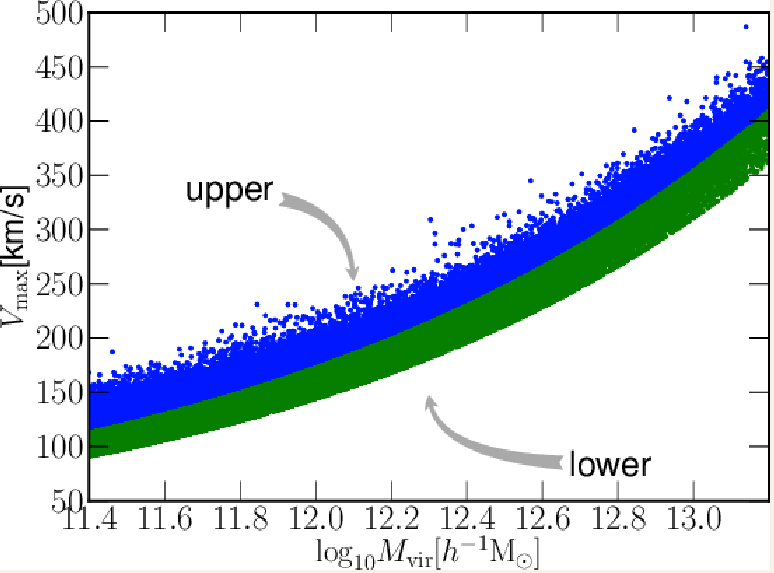
\includegraphics[width=0.5\columnwidth]{../plots/plaecholder}\caption{\label{fig:vmax-mvir}Distribution of halo mass and maximum circular
velocity at $z=0.0$ for halos\textcolor{black}{{} from the Bolshoi
simulation.} The blue dots represent halos whose observed maximum
circular velocity, $V_{{\rm max,obs}}$, is greater than $\overline{V}_{{\rm max}}$,
while the green dots are the ones with smaller $V_{{\rm max,obs}}$
than $\overline{V}_{{\rm max}}$. The boundary between blue and green
dots correspond to $\overline{V}_{{\rm max}}$ computed from Eq. \ref{eq:vmax-mvir}.}
\end{figure}


\textcolor{red}{To begin with, we split the sample of halos described
in Section 2 into a sequence of virial mass bins from high mass to
low mass, chosen such that there are the same numbers of halos in
each bin. We select 200000 halos for each bin for the halo sample
from the MultiDark simulation and 25000 halos for the Bolshoi simulation.
}This process is reminiscent of an abundance matching procedure (cite
XXX). We then further split each bin into two subsamples with their
observed $V_{{\rm max,obs}}$ greater than (denoted by ``upper'')
or less than (denoted as ``lower'') $\overline{V}_{{\rm max}}$.
Fig. \ref{fig:vmax-mvir} shows the distribution of halo mass and
maximum circular velocity classified into ``upper'' (blue dots)
and ``lower'' (green dots) samples as an example. Note that the
number of halos in ``upper'' and ``lower'' subsamples\textcolor{black}{{}
are }almost equal for any halo mass bins. This selection ensures that
both the upper and lower subsamples have the same mean halo mass.
Therefore, in the absence of an additional $V_{{\rm max}}$ dependence
on clustering, these samples should have the same clustering properties.\textcolor{red}{{}
Note that this would not be true if we had simply split the sample
along $V_{{\rm max}}$, since the two resulting subsamples would have
different mean halo masses. }


\subsection{Halo Bias}

In order to measure halo biases, we first compute halo-matter cross
correlation functions for each subsample. We used cross correlation
functions to reduce the shot noise effect on the error. Here, instead
of using full DM particles, we subsample $10^{6}$ particles to compute
the cross correlation functions and matter auto correlation functions.
Then, we define a linear bias: 
\begin{equation}
b_{{\rm lin}}=\sum_{i}(\xi_{hm}(r_{i})/\xi_{mm}(r_{i}))/N_{{\rm bin}},
\end{equation}
where $\xi_{hm}$ and $\xi_{mm}$ are halo-matter and matter-matter
correlation functions and we take the average of the ratio on $r$
from $10h^{-1}{\rm Mpc}$ to $20h^{-1}{\rm Mpc}$, which contains
20 bins in total. 

Fig. \ref{fig:linear-bias} shows linear biases as a function of halo
mass by splitting each sample into ``upper'' and ``lower'' subsamples.
For large halo masses, the ``lower'' subsamples have larger linear
biases than the ``upper'' subsamples. This result is consistent
with the result discussed in Ref. XXX(Dalal et al. 2008). For low
halo masses, the ``upper'' subsamples have larger linear biases
than the ``lower'' subsamples. Those halos, which have larger maximum
circular velocities than $\overline{V}_{{\rm max}}$, are the ones
which are supposed to grow into larger mass halos, but somehow the
mass growth is suppressed due to a tidal field {[}XXX: Wang et al.
+ Wetzel et al. 2014{]}. This is why those halos in the ``upper''
subsamples cluster more strongly than the ones in the ``lower''
subsamples. As halo mass decreases, the difference in linear bias
between the ``upper'' and ``lower'' subsamples increases up to
$\sim40\%$. On the low mass end, there is a drop in the ratio of
the linear biases. As we see no physical reasons, consider that this
is a resolution effect and suggest that the condition required for
completeness is more stringent {[}XXX: Peter's paper{]}.

\begin{figure}
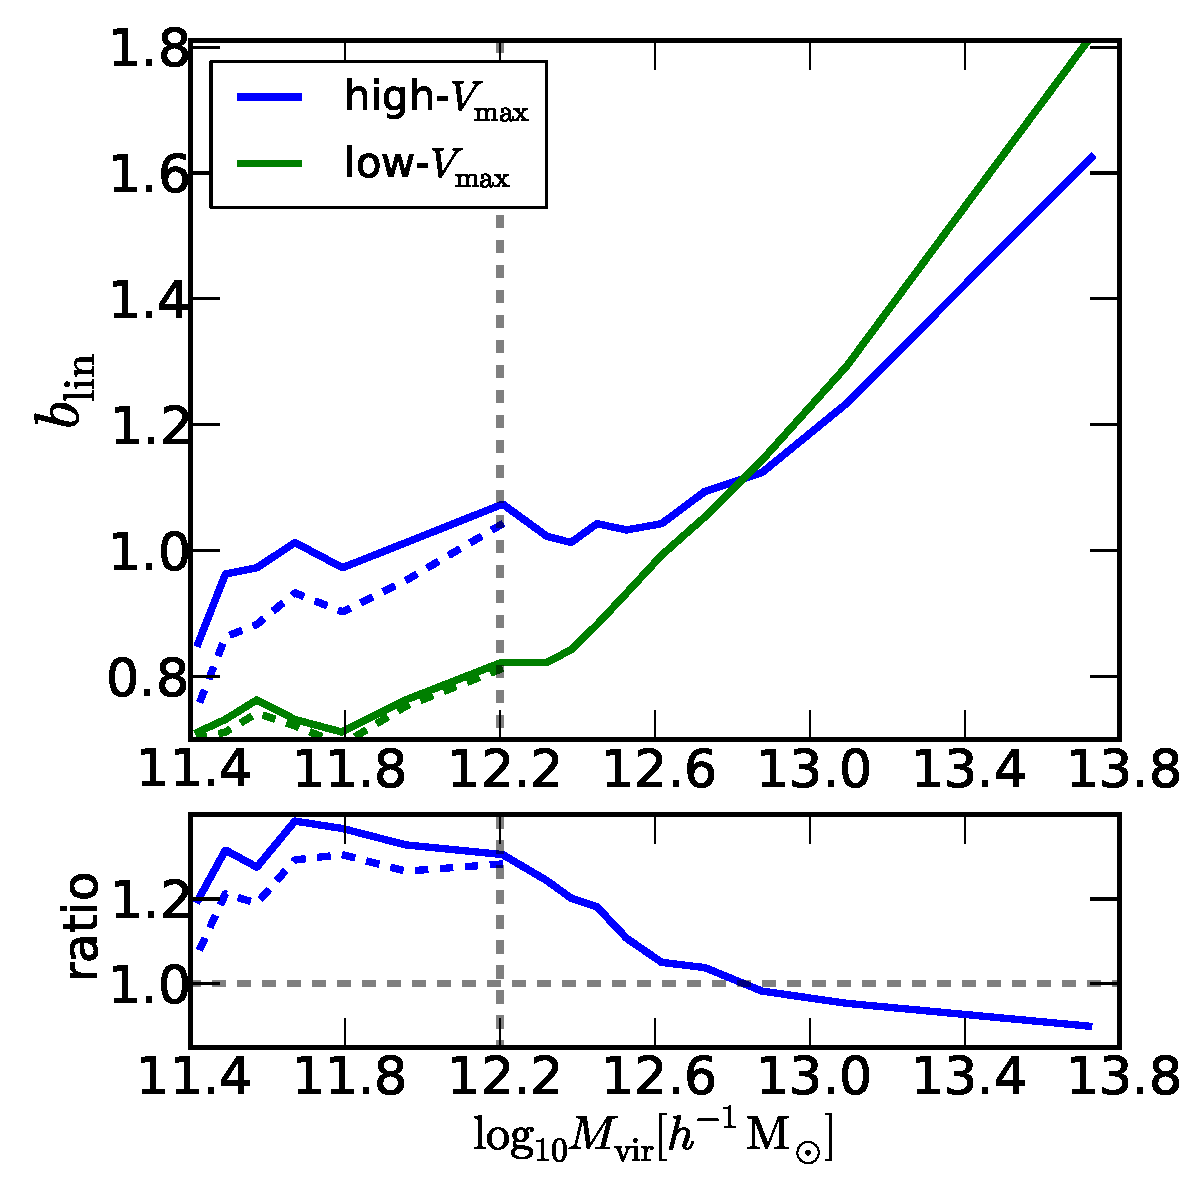
\includegraphics[width=0.5\columnwidth]{../plots/linearBias_wang}

\caption{\label{fig:linear-bias}Upper panel: Linear bias at $z=0.0$ as a
function of halo mass from the Bolshoi simulation (circle points)
and the MultiDark simulation (triangle points). The blue circles correspond
to a linear bias for halos whose maximum circular velocities are greater
than $\overline{V}_{{\rm max}}$ (called ``upper'' samples in the
text), while the green circles correspond to halos whose maximum circular
velocities are smaller than $\overline{V}_{{\rm max}}$ (called ``lower''
samples). Lower panel: Ratio of linear biases between ``upper''
(i.e., $V_{{\rm max}}>\overline{V}_{{\rm max}}$) and ``lower''
(i.e., $V_{{\rm max}}<\overline{V}_{{\rm max}}$) samples from the
Bolshoi simulation and the MultiDark simulation. As halo masses decrease,
the difference on linear bias between ``upper'' and ``lower''
samples becomes larger up to 40\%. .}
\end{figure}


Although halo biases are constant on large scales, halo biases on
small scales are scale-dependent (XXX:reference). We explore whether
the ``upper'' and ``lower'' subsamples have different scale-dependence
in small scale halo biases. In order to explore this, we take the
ratio of the cross correlation functions between the ``upper'' and
``lower'' subsamples and normalize it with their linear biases.
Fig. \ref{fig:small-scale} shows the ratios for several mass bins.
The first three mass bins labeled in the figure, ${\rm log_{10}M[h^{-1}{\rm M_{\odot}}]=11.7,12.0,12.2}$,
are from the Bolshoi simulation, and the last two mass bins, ${\rm log_{10}M[h^{-1}{\rm M_{\odot}}]=12.7,13.1}$,
are from the MultiDark simulation. The ``upper'' and ``lower''
subsamples have very different scale-dependence, especially around
1 to 2$h^{-1}{\rm Mpc}$. Furthermore, the difference on small scales
becomes larger for lower halo mass samples\textcolor{black}{. This
implies that those low mass halos in the ``upper'' subsamples cluster
strongly and are likely to live in hot environments near massive halos.}

Up until present, we have used both host halos and ejected halos to
compute halo biases. Both types of halos are identified as distinct
halos at $z=0$. Ejected halos, however, are halos which were identified
as part of more massive halos at one or more occasions in the past,
but were ejected and now exist at a host halo at $z=0$. Those ejected
halos tend to exist around more massive halos (any reference?), and
only some of them may be gravitationally bound to other more massive
halos. Therefore, the effect on scale-dependent biases may be caused
by those ejected halos. To test this, we compute halo-matter cross
correlation functions without the ejected halos. Similar to Fig. \ref{fig:linear-bias},
we first compare linear biases as a function of halo mass. We observe
that the ratios of linear biases between the ``upper'' and ``lower''
subsamples are suppressed to\textcolor{red}{{} $\sim25\%$}. Next, we
compare cross correlation functions on small scales, as shown in Fig.
\ref{fig:eject}, similar to what was done in Fig. \ref{fig:small-scale}.
Fig. \ref{fig:eject} only shows the results for low mass halos from\textcolor{black}{{}
the Bolshoi simulation. This is because} we do not find many ejected
halos in the MultiDark simulation due to its mass resolution. \textcolor{black}{Once
the ejected halos have been removed, the deviation of the halo bias
on small scales is greatly reduced. }This implies an intimate connection
between assembly bias and subhalo back-splashing.

We conclude that halos which have different $V_{{\rm max}}$ cluster
differently even when those halos have the same virial mass. In particular,
the scale-dependence of halo biases on small scales is significantly
different, which is mainly caused by the ejected halos. 

\begin{figure}[H]
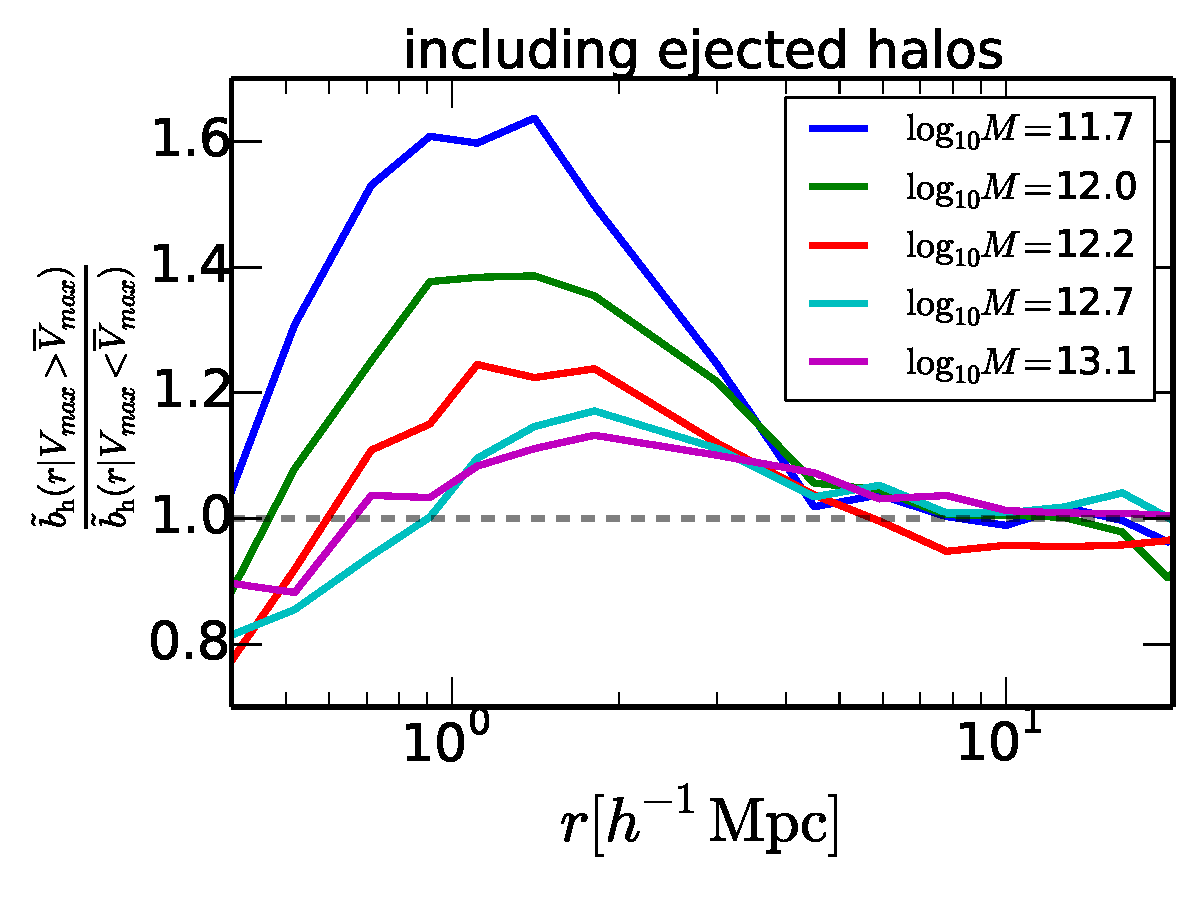
\includegraphics[width=0.8\columnwidth]{../plots/Both_smallScale_wang_log}

\caption{\label{fig:small-scale}Ratio of halo-matter cross correlation functions
between ``upper'' and ``lower'' subsamples normalized by their
linear biases. The plots are from the Bolshoi simulation and the MultiDark
simulation at $z=0$. Each line corresponds to different halo mass
bins labeled in the plots. The top three lines that correspond to
low mass halos are computed from halos in the Bolshoi simulation,
while the bottom lines are from the MultiDark simulation. Those plots
show that ``upper'' and ``lower'' subsamples have different scale-dependence
on small scales and the relative scale-dependence between those subsamples
increases smoothly with decreasing halo mass. }


\end{figure}


\begin{figure}[H]
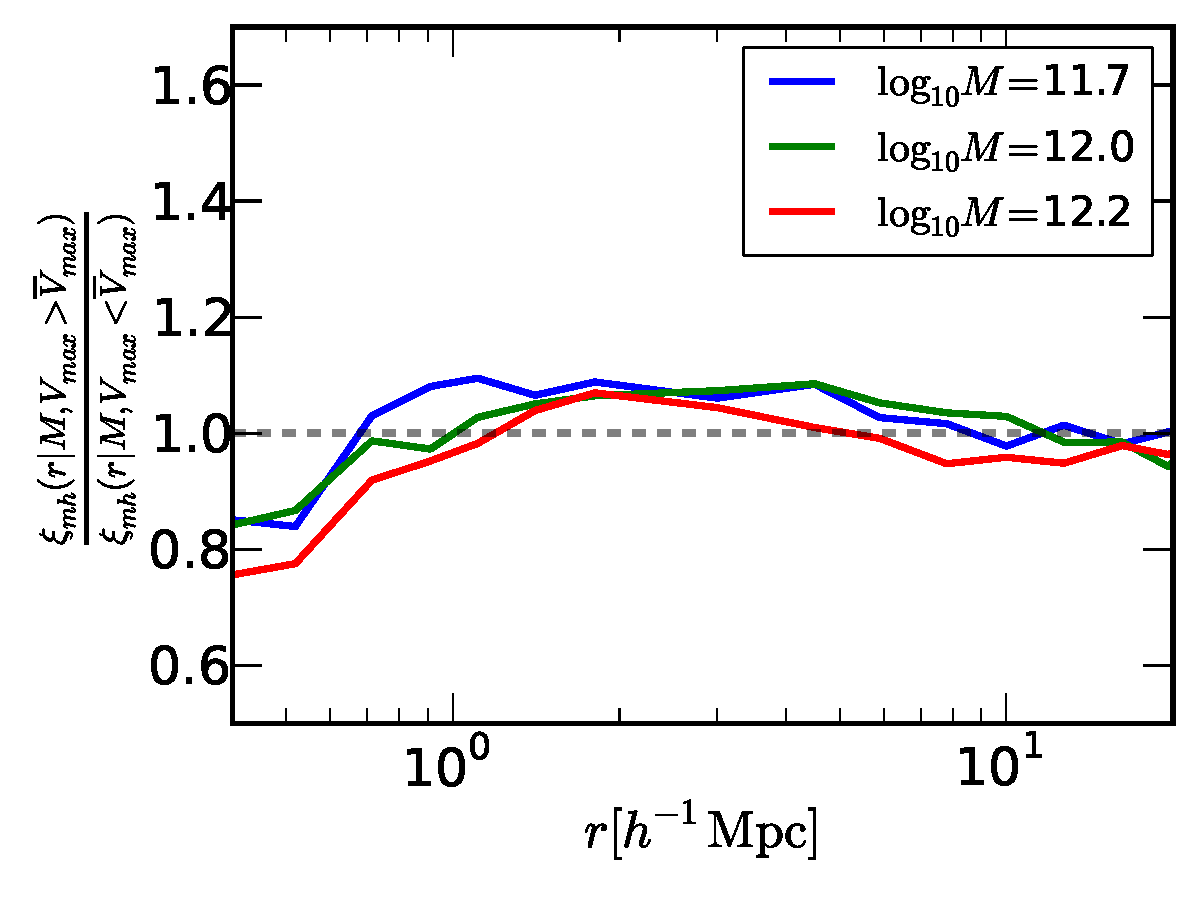
\includegraphics[width=0.5\columnwidth]{../plots/Bolshoi_smallScale_wang_log_eje}

\caption{\label{fig:eject}The same figures as Fig. \ref{fig:small-scale}
without ejected halos only from the Bolshoi simulation. As can be
seen by comparing these results to those in Fig. \ref{fig:small-scale},
the $V_{{\rm max}}$-dependence of halo bias on small scales is dramatically
reduced by excluding ejected subhalos. This implies an intimate connection
between assembly bias and subhalo back-splashing.}


\end{figure}


--use jackknife sampling to put error bars


\section{Applications}

In this section, we demonstrate \textcolor{black}{possible observational
relevances of the results in the previous section to complement the
halo theory results. }We start with the abundance matching (citation?)
technique based on halo mass and the maximum circular velocity which
may make qualitatively different predictions for clustering of central
galaxies.


\subsection{Mvir-based v.s. Vmax-based}

In abundance matching, we assume a monotonic relation between galaxy
luminosity and one of the halo properties which represent the ``size''
of halos and assign the most luminous galaxy to the largest halo in
a hierarchical manner so that $n_{g}(>L)=n_{h}(>M_{{\rm vir}}/V_{{\rm max}})$
where $n_{g}(>L)$ and $n_{h}(>M_{{\rm vir}}/V_{{\rm max}})$ are
the number density of galaxies and halos which have larger luminosity
$L$ or halo mass/the maximum circular velocity $M_{{\rm vir}}/V_{{\rm max}}$
respectively. In practice, we rank order halos by $M_{{\rm vir}}$
or $V_{{\rm max}}$ and select $N$ halos for each bin from high to
low. This time, we only use halo sample from the Bolshoi simulation
and select 25000 halos for each bin.

Similar to the previous section, we compute halo-matter cross correlation
functions for the abundance matched samples by splitting halos into
a sequence of halo mass bins, $\overline{n}(M_{{\rm vir}})$, and
the maximum circular velocity bins, $\overline{n}(V_{{\rm max}})$,
chosen such that each bin has the same number of halos. We observe
that when we include ejected halos, the linear biases for the $V_{{\rm max}}$-samples
are larger than the ones for the $M_{{\rm vir}}$-samples by 5\%,
while the difference in linear biases is suppressed to 2\% by excluding
ejected halos. This result is consistent with the result in Sec. 3.2.
The magnitude of the difference, however, is smaller than the cases
of splitting the samples based on $\overline{V}_{{\rm max}}$. 

We also compare the cross correlation functions on small scales. Figure
\ref{fig:abundance_small} displays data in the same way as Figure
\ref{fig:small-scale} with the ejected halos on the left and without
the ejected halos on the right. When those samples contain ejected
halos, the $V_{{\rm max}}$-samples show very different scale-dependence
on halo bias than the $M_{{\rm vir}}$-samples do. This scale-dependent
feature becomes stronger as halo mass decreases. Without ejected halos,
the difference on small-scale biases between the $M_{{\rm vir}}$-
and $V_{{\rm max}}$- samples is reduced to $\sim5\%$, which is the
same order of magnitude as the case of Sec. 3.3 shown in Fig. \ref{fig:eject}.

\begin{figure}[H]
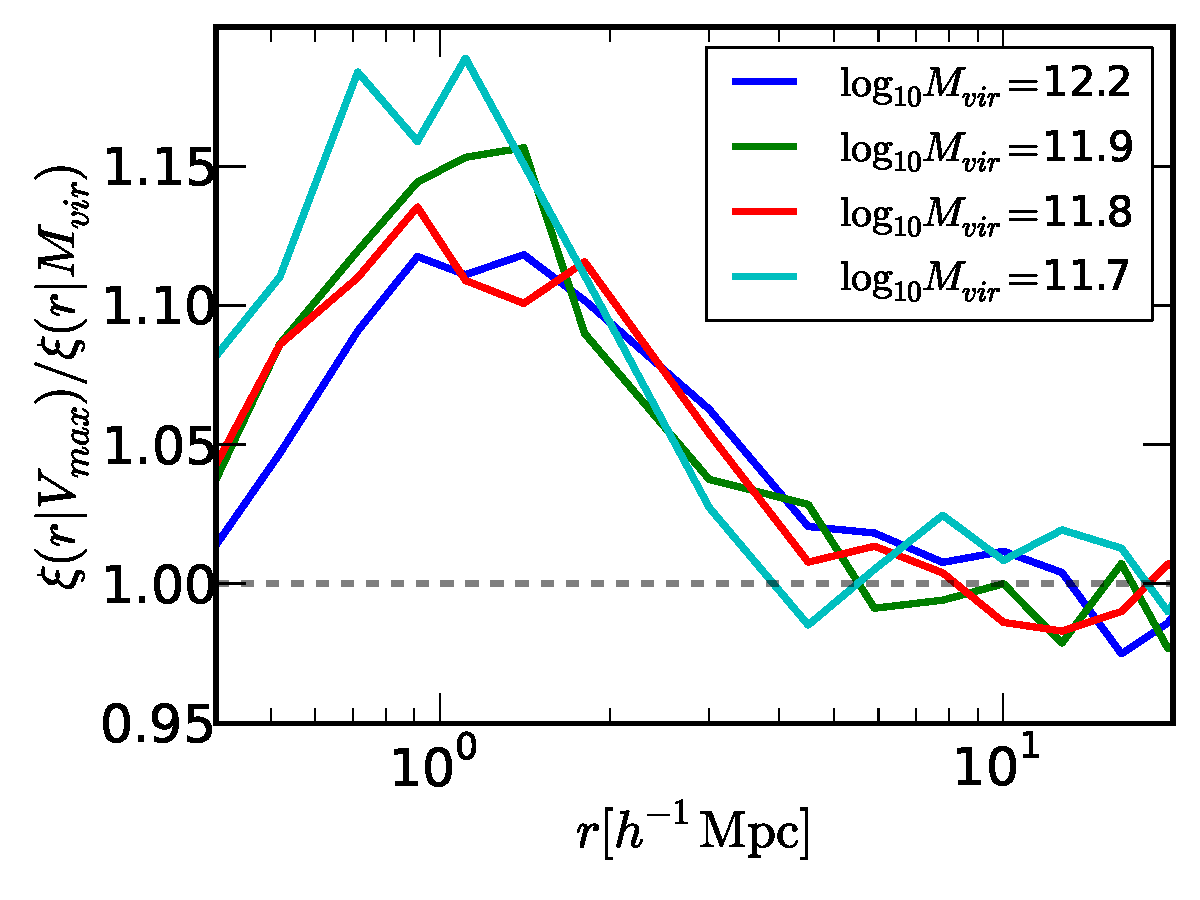
\includegraphics[width=0.5\columnwidth]{../plots/Bolshoi_andrew_smallScale}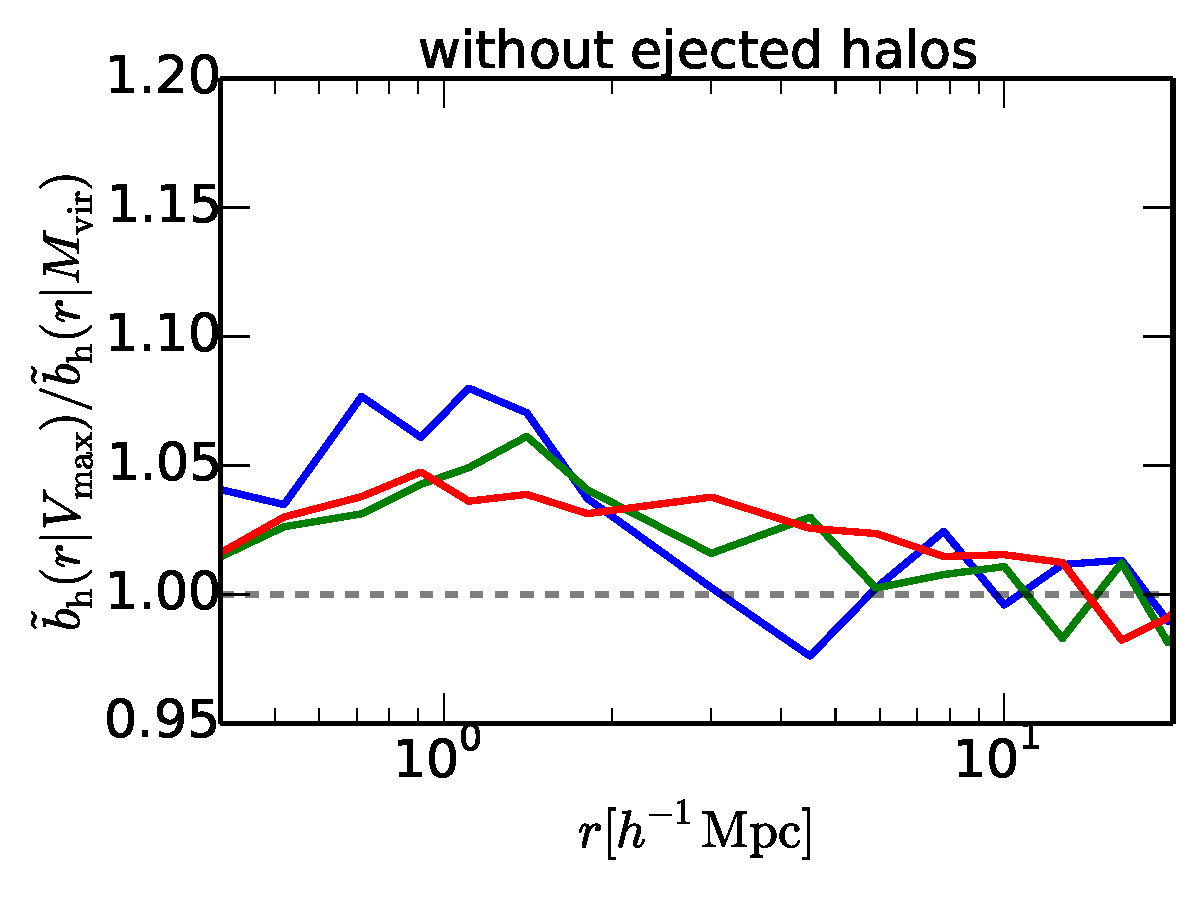
\includegraphics[width=0.5\columnwidth]{../plots/Bolshoi_andrew_smallScale_nonEj}

\caption{\label{fig:abundance_small}Ratio of halo-matter cross correlation
functions between$M_{{\rm vir}}$-based and $V_{{\rm max}}$-based
abundance matching samples with ejected halos (left) and without ejected
halos (right). The ratios are normalized by their linear biases. Each
line corresponds to different halo mass bins labeled in the plots.
With ejected halos, the halo biases computed from the $V_{{\rm max}}$-samples
have very different scale-dependence than the ones from the $M_{{\rm vir}}$-samples.
By removing those ejected halos, the difference is more or less removed.}
\end{figure}



\subsection{$\Delta\Sigma(r)$}

--Select a bin of Milky Way mass host halos, and select their number-density-matched
Vmax-selected equivalent. Use Peter Behroozi's stellar-to-halo mass
relation to estimate the stellar mass of the central galaxy that would
be found in these halos, then plot the halo-matter cross-correlation
as a function of scale, over-plotting the two results.

--want to show: We show that the galaxy-galaxy lensing signal of low-mass
centrals is impacted at the xxx-yyy\% level, in a highly scale-dependent
fashion, by the theoretical choice to empirically connect stellar
mass to either host halo Vmax or Mvir.


\section{Discussion}

In this paper, we explore additional dependence of halo clustering
on the maximum circular velocity of halos in addition to halo mass.
The maximum circular velocity is a measure of potential well depth
of halos, which determines the escape velocity of particles around
the halos and therefore determine the feedback efficiency for galaxy
formation.

Our result for linear bias is consistent with previous studies investigating
clustering dependence on other parameters such as formation time and
concentration (Ref. XXX). The result is expected since the maximum
circular velocity is tightly correlated with those parameters. In
high mass regime, halos with shallower potential well depth (hereafter,
PWD) cluster more strongly than the ones with deeper PWD. This is
nicely explained in terms of the statistics of peaks and peak curvature
of random Gaussian fields (XXX:Dalal et al. 2008). Two halos with
the same mass originated from the same peak height but different peak
curvature cluster differently because of their different environment.
The halos with shallower peak curvature tend to live in high density
region and therefore cluster more strongly. Since there is a correlation
between concentration and peak curvature, the maximum circular velocity
may correlate well with the curvature. In low mass regime, we observed
that halos with deeper PWD cluster more strongly and the dependence
of linear bias on PWD is stronger than in high mass regime. On low
mass end, the difference in linear bias for halos with deeper/shallower
PWD reaches to 40\%. This is consistent with previous works done for
formation time and concentration. Ref. XXX (vdB et al. 2014) shows
that the maximum circular velocity reaches to its current value at
early times than halo mass. This implies that low mass halos with
deeper PWD have higher halo mass at early times than the ones with
shallower PWD and their mass growth is suppressed at later times and
remain to be low mass halos. The suppressions of halo mass growth
is due to the strong tidal field generated in high density region
(Ref. XXX). So, those low mass halos with deeper PWD must live in
high density region and therefore cluster more strongly.

We also explore the scale dependence of halo assembly bias. On small
scales, halos with deeper PWD cluster much more strongly at $1-2h^{-1}{\rm Mpc}$
and this scale dependence feature on halo bias becomes stronger for
lower mass halos. This feature, however, is removed by excluding the
ejected halos. So, this scale dependence on assembly bias is due to
the ejected halos. Furthermore, the ejected halos clustering at $1-2h^{-1}{\rm Mpc}$
strongly means that they probably cluster around more massive host
halos. Ref. XXX (Wetzel et al. 2014) shows that those ejected halos
are subhalos which are gravitationally bound to more massive host
halos beyond the virial radius of those host halos and eventually
falling into the host halos after a few Gyrs. Those ejected halos
host satellite galaxies having more quiescent star formation rate
than a central galaxy. So, it is crucial to identify the ejected halos
and treat them differently when populate halos with galaxies, because
those host halos may host very different type of galaxies. In Section
4, we demonstrate that abundance matching techniques based on halo
mass and the maximum circular velocity give a very different scale
dependence on small scale halo bias with the ejected halos. It may
be observationally testable which parameter is better in use of the
abundance matching technique by identifying central galaxies and those
ejected satellite galaxies and measuring their halo bias.

One interesting question we did not explore in this paper is whether
those ejected halos are within the splashback radius of host halos,
which is the radius where accreted matter reaches its first apocenter
of orbit after turnaround. Several studies, which explore a more physically
motivated definition of halo radius, propose the idea of the splashback
radius, because XXX. If all the ejected halos are within the splashback
radius of host halos, it will more motivate to use splashback radius
as a halo radius and we do not need to consider treating the ejected
halos differently since they are naturally considered as subhalos.

In summary, we found a consistent trend to previous works in additional
dependence of linear bias on the maximum circular velocity for both
high/low mass halos. We also found that scale dependence of halo assembly
bias on small scales mostly come from the ejected halos, which suggest
to treat them differently in the methods to connect halo populations
to galaxy populations.

\bibliography{VmaxMvir}


\end{document}
